\chapter{Edo-Period Yōkai Culture: Catalogues, Ghost Stories and Kaidan}

\section{From fear to play}

The Edo period (1603--1868) transformed yōkai. A peaceful, urban, commercial and highly
literate society produced books, prints, games and theatre about monsters on a large scale.
Kagawa Masanobu (\emph{Edo no yōkai kakumei}, 2005) calls this the \textbf{``yōkai
revolution''}: yōkai moved from being objects of genuine fear to being \emph{characters}
for entertainment.

\begin{important}[Why the Edo period?]
\begin{itemize}
  \item \textbf{Print capitalism}: commercial woodblock publishing made illustrated books
        cheap; lending libraries spread them further.
  \item \textbf{Encyclopedic spirit}: Confucian ``investigation of things'' and natural
        history (\ja{本草学}, honzōgaku) encouraged cataloguing plants, animals, minerals,
        and monsters.
  \item \textbf{Urban leisure}: townspeople (\emph{chōnin}) had money and time for
        entertainment.
  \item \textbf{Declining belief}: as monsters became less believed in, they became more
        available for play and parody.
\end{itemize}
\end{important}

\section{Hyakumonogatari kaidankai}

\begin{definition}[Hyakumonogatari kaidankai]
The \emph{hyakumonogatari kaidankai} (\ja{百物語怪談会}, ``gathering for a hundred
weird tales'') was a popular game. Participants gathered at night and lit a hundred
wicks in a lamp (often with blue paper over it) in a back room. Each person told a
strange tale, then went alone to the back room, extinguished one wick and looked in a
mirror. When the last light went out, a real monster was supposed to appear.
\end{definition}

\begin{center}
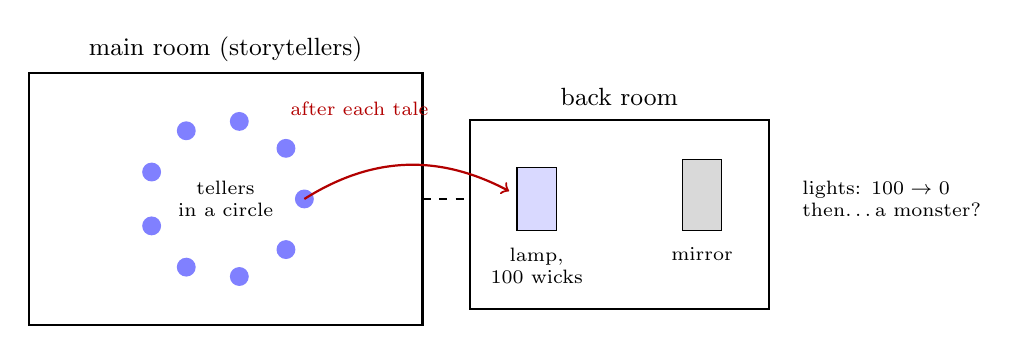
\begin{tikzpicture}
  % room layout
  \draw[thick] (0,0) rectangle (5,3.2);
  \draw[thick] (5.6,0.2) rectangle (9.4,2.6);
  \draw[thick, dashed] (5,1.6) -- (5.6,1.6);
  \node[font=\small] at (2.5,3.5) {main room (storytellers)};
  \node[font=\small] at (7.5,2.9) {back room};
  \foreach \a in {0,40,...,320} { \fill[blue!50] ({2.5+1.0*cos(\a)},{1.6+1.0*sin(\a)}) circle (0.12); }
  \node[font=\scriptsize, align=center] at (2.5,1.6) {tellers\\in a circle};
  \draw[fill=blue!15] (6.2,1.2) rectangle (6.7,2.0);
  \node[font=\scriptsize, align=center] at (6.45,0.75) {lamp,\\100 wicks};
  \draw[fill=gray!30] (8.3,1.2) rectangle (8.8,2.1);
  \node[font=\scriptsize] at (8.55,0.9) {mirror};
  \draw[->, thick, red!70!black] (3.5,1.6) to[bend left=30] (6.1,1.7);
  \node[font=\scriptsize, red!70!black] at (4.2,2.75) {after each tale};
  \node[font=\scriptsize, align=left, anchor=west] at (9.7,1.6) {lights: $100 \to 0$\\then\ldots a monster?};
\end{tikzpicture}
\end{center}

\begin{itemize}
  \item The game produced a whole genre of books, also called \emph{hyakumonogatari},
        collecting ``a hundred'' tales (\emph{Shokoku hyakumonogatari}, 1677).
  \item Many collections deliberately stopped at 99 tales, to avoid summoning the monster.
  \item Foster reads the game as a kind of \emph{ritual play}: it summoned fear in a
        controlled way, and its rules (counting, lights) mimic scientific experiment.
\end{itemize}

\section{Toriyama Sekien's catalogues}

\textbf{Toriyama Sekien} (\ja{鳥山石燕}, 1712--1788), a painter of the Kanō school and
teacher of the ukiyo-e master Utamaro, published four illustrated yōkai encyclopedias
between 1776 and 1784.

\begin{center}
\begin{tabular}{llp{7.5cm}}
\toprule
Title & Year & Notes \\
\midrule
\emph{Gazu hyakki yagyō} \ja{画図百鬼夜行} & 1776 & ``Illustrated Night Parade of a Hundred Demons''; well-known folk yōkai (kappa, tengu, kitsune) \\
\emph{Konjaku gazu zoku hyakki} \ja{今昔画図続百鬼} & 1779 & continuation \\
\emph{Konjaku hyakki shūi} \ja{今昔百鬼拾遺} & 1781 & ``gleanings''; more literary and invented figures \\
\emph{Hyakki tsurezure bukuro} \ja{百器徒然袋} & 1784 & mostly object-yōkai (tsukumogami), many invented by Sekien as puns \\
\bottomrule
\end{tabular}
\end{center}

\begin{itemize}
  \item \textbf{Format}: one yōkai per page, a picture with a name and often a short,
        witty caption. The format resembles a natural-history encyclopedia: the creatures
        are isolated from narrative, ready to be collected.
  \item \textbf{Invention}: many entries are Sekien's own inventions based on wordplay,
        poetry and classical allusions. Some ``traditional'' yōkai known today exist only
        because Sekien drew them, and Mizuki Shigeru later redrew them.
  \item \textbf{Legacy}: Sekien's images define the canonical look of many yōkai. His
        books are the direct ancestors of yōkai field guides, Mizuki's encyclopedias, and
        Pokémon's Pokédex (Week 12).
\end{itemize}

\begin{example}[A Sekien pun]
The \emph{Hyakki tsurezure bukuro} ends with yōkai that are household tools, often
punning on titles of classical texts (the book's title itself parodies the
\emph{Tsurezuregusa}, a 14th-century essay collection). Understanding Sekien requires
literacy in the classics: his audience was educated and enjoyed the jokes.
\end{example}

\begin{center}
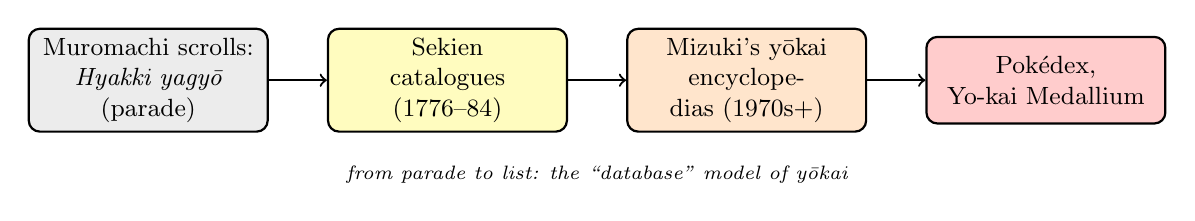
\begin{tikzpicture}[b/.style={draw, thick, rounded corners, align=center, font=\small, text width=2.8cm, minimum height=1.1cm}]
  \node[b, fill=gray!15] (scroll) at (0,0) {Muromachi scrolls:\\\emph{Hyakki yagyō} (parade)};
  \node[b, fill=yellow!25] (sekien) at (3.8,0) {Sekien\\catalogues\\(1776--84)};
  \node[b, fill=orange!20] (mizuki) at (7.6,0) {Mizuki's yōkai encyclopedias (1970s+)};
  \node[b, fill=red!20] (poke) at (11.4,0) {Pokédex,\\Yo-kai Medallium};
  \draw[->, thick] (scroll) -- (sekien);
  \draw[->, thick] (sekien) -- (mizuki);
  \draw[->, thick] (mizuki) -- (poke);
  \node[font=\scriptsize\itshape] at (5.7,-1.2) {from parade to list: the ``database'' model of yōkai};
\end{tikzpicture}
\end{center}

\section{Kaidan: strange tales}

\begin{definition}[Kaidan]
\emph{Kaidan} (\ja{怪談}, ``strange talk'') are tales of the supernatural, especially ghost
stories. Many Edo kaidan were adapted from Chinese collections of the strange (Ming
dynasty \emph{Jiandeng xinhua}), relocated to Japanese settings.
\end{definition}

\begin{itemize}
  \item \textbf{Asai Ryōi}, \emph{Otogibōko} (1666): includes the source of \emph{Botan dōrō}.
  \item \textbf{Ueda Akinari}, \emph{Ugetsu monogatari} (\ja{雨月物語}, ``Tales of Moonlight
        and Rain'', 1776): nine elegant tales, e.g.\ ``The Kibitsu Cauldron'' (a betrayed
        wife's vengeful ghost) and ``The Lust of the White Serpent''. Adapted by Mizoguchi
        Kenji in the film \emph{Ugetsu} (1953).
  \item \textbf{Lafcadio Hearn} (Koizumi Yakumo) retold kaidan in English in
        \emph{Kwaidan} (1904), which shaped Western images of Japanese ghosts (Week 7).
\end{itemize}

\section{Yotsuya Kaidan: Oiwa}

\textbf{Tsuruya Nanboku IV}'s kabuki play \emph{Tōkaidō Yotsuya kaidan} (\ja{東海道四谷怪談},
1825) is the most famous Japanese ghost story.

\subsection{Plot outline}

\begin{enumerate}
  \item The masterless samurai (\emph{rōnin}) \textbf{Iemon} murders Oiwa's father to
        stay married to her.
  \item A wealthy neighbour's granddaughter falls for Iemon. Her family sends Oiwa a
        ``medicine'' that is actually poison: it disfigures her face (one eye droops, her
        hair falls out in bloody clumps as she combs it in a famous scene).
  \item Iemon, wanting to remarry, arranges for a man to seduce Oiwa so that he can
        divorce her. Learning the truth, Oiwa dies cursing Iemon (accidentally cutting her
        throat on a sword).
  \item Iemon nails Oiwa's body and that of a murdered servant to two sides of a door and
        throws it in a river.
  \item Oiwa's ghost haunts Iemon: on his wedding night he sees her face on his bride and
        kills her; the door with the two corpses floats up as he fishes (``the door
        flip'', \ja{戸板返し}); her face appears in a paper lantern (\ja{提灯抜け}). Iemon
        is finally killed.
\end{enumerate}

\begin{important}[Reading Oiwa]
\begin{itemize}
  \item The play was performed together with \emph{Chūshingura} (the loyal 47 rōnin):
        Iemon is a bad samurai, an anti-hero who inverts the ideals of loyalty.
  \item Oiwa's ghost is a \emph{woman's revenge against a male betrayer}: the jealous female
        spirit of the Heian period becomes a social critique of samurai men.
  \item Spectacle: stage tricks (quick changes, trap doors, the lantern) made kabuki ghosts
        a technological entertainment, much as special effects would later.
  \item Iconography: the disfigured face, long dishevelled hair and white burial robe
        became the standard image of the female yūrei, leading to Sadako (Week 10).
\end{itemize}
\end{important}

\begin{aside}
Actors still visit Oiwa's shrine in Yotsuya (Tokyo) before staging the play or filming an
adaptation, to ask permission and avoid her curse. Theatre people take Oiwa seriously.
\end{aside}

\section{Botan dōrō: the peony lantern}

\emph{Botan dōrō} (\ja{牡丹燈籠}, ``The Peony Lantern''), from a Chinese tale, was retold as
a famous \emph{rakugo} storytelling piece by San'yūtei Enchō in the 1860s.

\begin{itemize}
  \item On the night of Obon, the young samurai \textbf{Hagiwara Shinzaburō} sees a
        beautiful woman, Otsuyu, and her maid passing by carrying a lantern decorated with
        peonies. They become lovers; she visits every night.
  \item A neighbour peeps through the wall and sees Shinzaburō embracing a skeleton.
  \item A priest gives him protective talismans to paste over the doors and a Buddhist
        image to wear. The ghost cannot enter and weeps outside.
  \item Shinzaburō's servants, bribed by the ghost, remove the talisman. He is found dead,
        clutching a skeleton.
\end{itemize}

\begin{center}
\begin{tabular}{p{3cm}p{5cm}p{5cm}}
\toprule
 & \emph{Yotsuya kaidan} & \emph{Botan dōrō} \\
\midrule
Ghost & Oiwa, betrayed wife & Otsuyu, lovesick woman \\
Motive & revenge (urami) & love/desire beyond death \\
Look & disfigured, terrifying & beautiful (to the lover); a skeleton (to others) \\
Medium & kabuki (1825) & Chinese tale $\to$ rakugo (1860s) \\
Moral & punishment of a betrayer & danger of passion; Buddhist protection fails through human greed \\
\bottomrule
\end{tabular}
\end{center}

\section{The yūrei image}

The classic Japanese ghost has no feet. This is often credited to the painter \textbf{Maruyama
Ōkyo} (1733--1795), whose ghost painting shows a pale woman fading into nothing below the
waist (earlier examples exist). By the late Edo period the iconography was fixed:

\begin{itemize}
  \item white burial kimono (\ja{死装束}), folded right over left (the reverse of the living);
  \item a white triangular headband (\ja{天冠}, tenkan);
  \item long, unbound black hair;
  \item hands hanging limply at the wrist, held in front;
  \item no feet, floating; accompanied by blue-white will-o'-the-wisps (\ja{人魂}, hitodama).
\end{itemize}

\section*{Summary}
\begin{itemize}
  \item The Edo ``yōkai revolution'': commercial printing and natural history turned yōkai
        into characters for play.
  \item Hyakumonogatari kaidankai: a storytelling game that produced a genre of books.
  \item Toriyama Sekien's four catalogues (1776--84) created the encyclopedic, one-per-page
        ``database'' format and invented many yōkai.
  \item Kaidan: Ueda Akinari's \emph{Ugetsu}; \emph{Yotsuya kaidan} (Oiwa, 1825);
        \emph{Botan dōrō}.
  \item The standard yūrei image (white robe, long hair, no feet) took shape in the Edo period.
\end{itemize}
